% !TEX program = pdflatex
\documentclass[11pt, a4paper]{article}

% ─── Packages ────────────────────────────────────────────────────────────────
\usepackage[utf8]{inputenc}
\usepackage[T1]{fontenc}
\usepackage{lmodern}
\usepackage[margin=2.5cm]{geometry}
\usepackage{amsmath, amssymb, amsthm}
\usepackage{booktabs}
\usepackage{enumitem}
\usepackage{hyperref}
\usepackage{cleveref}
\usepackage{xcolor}
\usepackage{graphicx}
\usepackage[font=small, labelfont=bf]{caption}
\usepackage{subcaption}
\usepackage{microtype}
\usepackage{natbib}
\usepackage{authblk}
\usepackage{lineno}

\hypersetup{
    colorlinks=true,
    linkcolor=blue!70!black,
    citecolor=green!50!black,
    urlcolor=blue!60!black,
}

% ─── Title ───────────────────────────────────────────────────────────────────
\title{%
    \textbf{Epistemic Gated Bootstrapped DQN (EG-BDQN):} \\[0.3em]
    \large Preliminary Findings on Budget-Constrained Oracle Supervision \\
    for Guided Exploration in Discrete Reasoning Tasks%
}

\author{Vaibhav Jain}
\affil{vaja00001@uni-saarland.de}
\date{April 2026 \\ {\small \textit{Preliminary Report --- Not Peer-Reviewed}}}

\begin{document}
\linenumbers
\maketitle

% ─────────────────────────────────────────────────────────────────────────────
\section{Abstract}
% ─────────────────────────────────────────────────────────────────────────────

Integrating expert oracles---such as Large Language Models (LLMs)---as interactive advisors in Reinforcement Learning (RL) is a promising avenue for solving sparse-reward and hard-exploration tasks. However, querying high-latency, high-cost external models at every timestep is computationally prohibitive. Na\"ive gating mechanisms based on raw policy entropy conflate environmental stochasticity (aleatoric uncertainty) with genuine agent ignorance (epistemic uncertainty), leading to wasteful budget expenditure. Furthermore, injecting externally generated actions into standard RL pipelines risks non-stationarity and credit assignment failures.

We present \textbf{Epistemic Gated Bootstrapped DQN (EG-BDQN)}, a framework that formulates oracle assistance as a budgeted querying problem. By leveraging ensemble disagreement across the Q-network heads native to Bootstrapped DQN, the system estimates epistemic value uncertainty and gates oracle queries to states where the agent genuinely lacks knowledge. DQN's off-policy replay buffer absorbs oracle demonstrations without corrupting the agent's internal credit assignment.

This report details two rounds of preliminary experiments on the BabyAI \texttt{GoToDoor-v0} environment using a heuristic bot as a surrogate oracle. The first round documents \textit{premature epistemic gate closure}, wherein the gating mechanism shuts off supervision before the value function achieves robustness. Remediation via mixture gating resolved this issue but uncovered a deeper failure: upon budget exhaustion, performance collapses sharply---a signature of \textit{oracle-induced covariate shift}. We provide a theoretical diagnosis grounding this collapse in the DAgger framework, analyze the causal mechanisms, and outline a concrete roadmap toward safe oracle-to-autonomous policy transfer.


% ─────────────────────────────────────────────────────────────────────────────
\section{Related Work}
% ─────────────────────────────────────────────────────────────────────────────

This research bridges active imitation learning, epistemic exploration, and neuro-symbolic reinforcement learning. We position our work against three primary threads in the literature:

\paragraph{Uncertainty-Gated Oracle Assistance.} 
The integration of Large Language Models (LLMs) as interactive agents has driven recent interest in budgeted guidance. Most closely aligned with our work is \textit{When to ASK: Uncertainty-Gated Language Assistance for Reinforcement Learning} (2026), which utilizes epistemic uncertainty to trigger LLM interventions, minimizing high-cost API calls in out-of-distribution states. Similarly, works exploring LLMs for guiding exploration \citep{du2023guiding} or as zero-shot planners \citep{huang2022language, ichter2023do} often struggle with the latency of continuous querying. Our approach builds on the "When to ASK" paradigm but shifts the focus from on-policy actor-critic architectures---which suffer from severe credit assignment failures when injected with external actions---to an off-policy value-absorption framework.

\paragraph{Epistemic Exploration in Value-Based RL.}
Distinguishing between environmental stochasticity (aleatoric) and agent ignorance (epistemic) is crucial for budgeted querying. We build upon the foundational \textit{Deep Exploration via Bootstrapped DQN} \citep{osband2016deep}. While Osband et al. utilized Q-ensembles combined with randomized prior functions to drive deep, autonomous exploration, we repurpose the ensemble's variance strictly as a gating metric. By treating Q-head disagreement as an explicit trigger for external oracle queries, we effectively bound the exploration time required by traditional Bootstrapped DQN.

\paragraph{Demonstration Absorption and Covariate Shift.}
Learning from expert interventions without corrupting the autonomous policy is a well-documented challenge. \textit{Deep Q-learning from Demonstrations (DQfD)} \citep{hester2018deep} established the necessity of permanent demonstration retention (dual-buffers) combined with margin classification losses to anchor Q-values. However, relying on fixed expert data introduces transition-distribution failures. As established by the \textit{DAgger} framework \citep{ross2011reduction}, policies trained under expert-corrected state distributions often collapse when deployed autonomously due to covariate shift. Our observed failure modes actively engage with this DAgger-style distribution shift, positioning EG-BDQN as a testbed for solving covariate shift in dynamically gated, mixed-control neuro-symbolic systems.


% ─────────────────────────────────────────────────────────────────────────────
\section{Problem Formulation}
% ─────────────────────────────────────────────────────────────────────────────

We frame oracle integration as a problem of \textbf{Resource-Constrained Epistemic Exploration}. The agent seeks to maximize expected return subject to a hard, finite lifetime budget of $B$ total oracle queries. Let $c_t \in \{0,1\}$ indicate whether the oracle is queried at timestep $t$. The budget constraint is:
\begin{equation}
    \sum_{t=0}^{T} c_t \leq B.
    \label{eq:budget}
\end{equation}

Solving this problem requires addressing two critical bottlenecks:
\begin{enumerate}[leftmargin=*, label=(\roman*)]
    \item \textbf{Misclassification of Uncertainty.} Existing methods trigger queries using raw policy entropy $H(\pi(\cdot \mid s))$. This wastes budget on states with high aleatoric uncertainty (inherent transition noise) rather than targeting states where the agent legitimately lacks value-based knowledge.
    \item \textbf{Credit Assignment Contamination.} Injecting external actions into on-policy algorithms breaks the surrogate objective: the actor network receives falsely attributed gradient updates for the oracle's success, overestimating its own competence.
\end{enumerate}


% ─────────────────────────────────────────────────────────────────────────────
\section{Methodology}
% ─────────────────────────────────────────────────────────────────────────────

\subsection{Epistemic Uncertainty via BDQN Ensembles}

To optimize the query budget, interventions must be gated on the agent's ignorance of the reward landscape. We employ Bootstrapped DQN, which natively maintains an ensemble of $N$ Q-network heads sharing a common feature encoder. For the greedy action $a^* = \arg\max_a \bar{Q}(s,a)$, the unnormalized epistemic uncertainty is:
\begin{equation}
    U_{\text{raw}}(s, a^*) = \mathrm{Var}\bigl(Q_1(s, a^*),\; Q_2(s, a^*),\; \ldots,\; Q_N(s, a^*)\bigr).
    \label{eq:raw_uncertainty}
\end{equation}

\paragraph{Relative Normalization.}
As training progresses, the absolute magnitude of Q-values grows, which can artificially inflate raw variance. We normalize via the coefficient of variation:
\begin{equation}
    U_{\mathrm{ep}}(s, a^*) = \frac{\mathrm{Std}(Q_1, \ldots, Q_N)}{\bigl|\bar{Q}(s, a^*)\bigr| + \epsilon},
    \label{eq:normalized_uncertainty}
\end{equation}
where $\epsilon > 0$ prevents division by zero. A high $U_{\mathrm{ep}}$ signals that the ensemble disagrees on the value of the current greedy action, indicating epistemic ignorance.

\subsection{Off-Policy Credit Assignment}

We leverage the off-policy nature of Q-learning to absorb oracle demonstrations without credit assignment contamination:
\begin{itemize}[leftmargin=*]
    \item \textbf{Gated Execution.} In state $s_t$, the system evaluates $U_{\mathrm{ep}}(s_t, a^*)$. If $U_{\mathrm{ep}} \leq \tau_t$, the ensemble executes its greedy action ($c_t = 0$). If $U_{\mathrm{ep}} > \tau_t$, the oracle is queried ($c_t = 1$).
    \item \textbf{Buffer Injection.} Regardless of which agent acts, the transition $(s_t, a_t, r_t, s_{t+1})$ is stored in the shared replay buffer $\mathcal{D}$.
    \item \textbf{Value-Based Learning.} Because DQN evaluates transitions independently of the behavior policy, the Q-heads learn the value of oracle-generated trajectories via standard TD updates. The agent benefits from oracle guidance without attributing gradient credit for generating those actions.
\end{itemize}

\subsection{Dynamic Percentile Thresholding}

Rather than a fixed threshold, we maintain a rolling buffer of recent $U_{\mathrm{ep}}$ values and set the gating threshold $\tau_t$ as the $(100 - x)$-th percentile of this buffer. This ensures that only the most uncertain states---relative to the agent's current calibration---trigger oracle queries. In our experiments, we set $x = 10$, querying the oracle when the current uncertainty falls in the top 10\% of recently observed values.

To prevent complete disconnection from supervision, we additionally employ a stochastic \textit{supervision floor}: with probability $p_{\mathrm{floor}} = 0.05 \cdot (B_{\mathrm{remaining}} / B)$, the oracle is queried regardless of $U_{\mathrm{ep}}$, providing a budget-proportional minimum supervision rate that decays as the budget is consumed.


% ─────────────────────────────────────────────────────────────────────────────
\section{Experimental Setup}
\label{sec:setup}
% ─────────────────────────────────────────────────────────────────────────────

\subsection{Environment and Oracle}

All experiments use the \texttt{BabyAI-GoToDoor-v0} environment, which requires navigating a grid-world to reach a target door specified by a natural-language mission string. Observations are compact $7 \times 7 \times 3$ grids processed by a CNN encoder; mission strings are tokenized via hash-based bag-of-words embeddings. The surrogate oracle is the BabyAI built-in heuristic bot, which provides optimal actions. This isolates the gating mechanism from language-model-specific noise while faithfully simulating the budgeted query setting.

\subsection{Architecture}

The BDQN network consists of a shared CNN encoder (three convolutional layers with $2 \times 2$ kernels), a mission embedding module (mean-pooled word embeddings, $d = 32$), a fusion layer ($d = 128$), and $N = 10$ independent two-layer Q-heads. Bernoulli bootstrap masking ($p = 0.5$) is applied per head during training to encourage ensemble diversity.

\subsection{Baselines}

We compare EG-BDQN against three baselines, each isolating a specific component of the framework:
\begin{enumerate}[leftmargin=*, label=(\roman*)]
    \item \textbf{Standard DQN} ($B = 0$): No oracle access, single Q-head. Establishes task difficulty.
    \item \textbf{Random Oracle Injection}: Uncertainty-gated, but injected actions are uniformly random rather than expert. Tests the value of expert advice \textit{per se}.
    \item \textbf{Budget-Matched Random Gating}: Expert oracle queried at random timesteps, consuming the same total budget $B$. Tests whether \textit{query timing} matters.
\end{enumerate}

\subsection{Training Details}

Training runs for $T = 100{,}000$ steps with budget $B = 5{,}000$ (except for the DQN baseline). We use Adam ($\eta = 3 \times 10^{-4}$), $\gamma = 0.99$, target network updates every $1{,}000$ steps, and $\epsilon$-greedy exploration decaying linearly from $1.0$ to $0.05$ over $30{,}000$ steps. All experiments are repeated across three random seeds (42, 123, 412), and we report 100-episode rolling mean returns.


% ─────────────────────────────────────────────────────────────────────────────
\section{Preliminary Results and Insights}
\label{sec:results}
% ─────────────────────────────────────────────────────────────────────────────

\subsection{Round 1: Premature Epistemic Gate Closure}

\Cref{tab:results_r1} summarizes the terminal performance from our first round of experiments. The central finding is negative but instructive: \textbf{EG-BDQN underperforms the budget-matched random gating baseline.} Random gating achieves a rolling mean return of approximately $0.65$, while EG-BDQN reaches $0.35$--$0.42$ depending on the thresholding variant, only modestly above the no-oracle DQN floor ($\sim 0.18$).

\begin{table}[h]
    \centering
    \caption{Round 1: Terminal rolling mean return (100-episode window) at $T = 100{,}000$ steps, seed 42. Budget $B = 5{,}000$ for all oracle-assisted conditions except DQN.}
    \label{tab:results_r1}
    \begin{tabular}{@{} l c c c @{}}
        \toprule
        \textbf{Condition} & \textbf{Rolling Mean Return} & \textbf{Queries Used} & \textbf{Budget Remaining} \\
        \midrule
        Standard DQN (no oracle) & $\sim 0.18$ & 0 & --- \\
        EG-BDQN (budget-aware) & $\sim 0.42$ & 3{,}994 & 1{,}006 \\
        EG-BDQN (no budget scaling) & $\sim 0.35$ & 5{,}000 & 0 \\
        Random Gating (budget-matched) & $\sim 0.65$ & 5{,}000 & 0 \\
        \bottomrule
    \end{tabular}
\end{table}

The underperformance is not attributable to ``oracle forgetting'' from the replay buffer, nor to insufficient budget. Instead, we identify a \textbf{self-reinforcing failure cascade} rooted in the interaction between the gating mechanism and the shared-encoder ensemble:

\begin{enumerate}[leftmargin=*, label=\textbf{(\arabic*)}]
    \item \textbf{Rapid early learning.} The epistemic gate correctly identifies high-uncertainty states and queries the oracle. The agent learns rapidly from these high-value demonstrations.
    \item \textbf{Ensemble disagreement collapses.} As oracle-supplied transitions reduce uncertainty, the $N$ Q-heads converge. The shared feature encoder amplifies this convergence, suppressing inter-head variance.
    \item \textbf{The gate prematurely closes.} With $U_{\mathrm{ep}}$ collapsing across the state space, the percentile-based threshold $\tau_t$ drops. The agent appears confident \textit{everywhere}, and queries cease---even though the value function is not yet robust.
    \item \textbf{Replay buffer homogenization.} Without ongoing oracle injections, the buffer becomes dominated by self-generated, correlated trajectories.
    \item \textbf{Correlated Q-head errors and bootstrapping amplification.} The shared encoder causes all heads to develop correlated errors. DQN bootstrapping amplifies these self-consistent mistakes rather than correcting them.
    \item \textbf{Policy drift.} Oracle transitions become too weak a corrective signal. The policy drifts and performance decays steadily.
\end{enumerate}

This failure mode is \textit{self-reinforcing}: gate closure reduces data diversity, which increases correlated errors, which further suppresses $U_{\mathrm{ep}}$, which keeps the gate closed. Meanwhile, the budget-matched random gating baseline avoids this cascade because it \textbf{never fully disconnects from expert supervision}---oracle queries are distributed uniformly across training, maintaining a minimum supervision floor that preserves replay diversity and limits correlated Q-head errors.

\begin{figure}[h]
    \centering
    \begin{subfigure}[b]{0.48\textwidth}
        \centering
        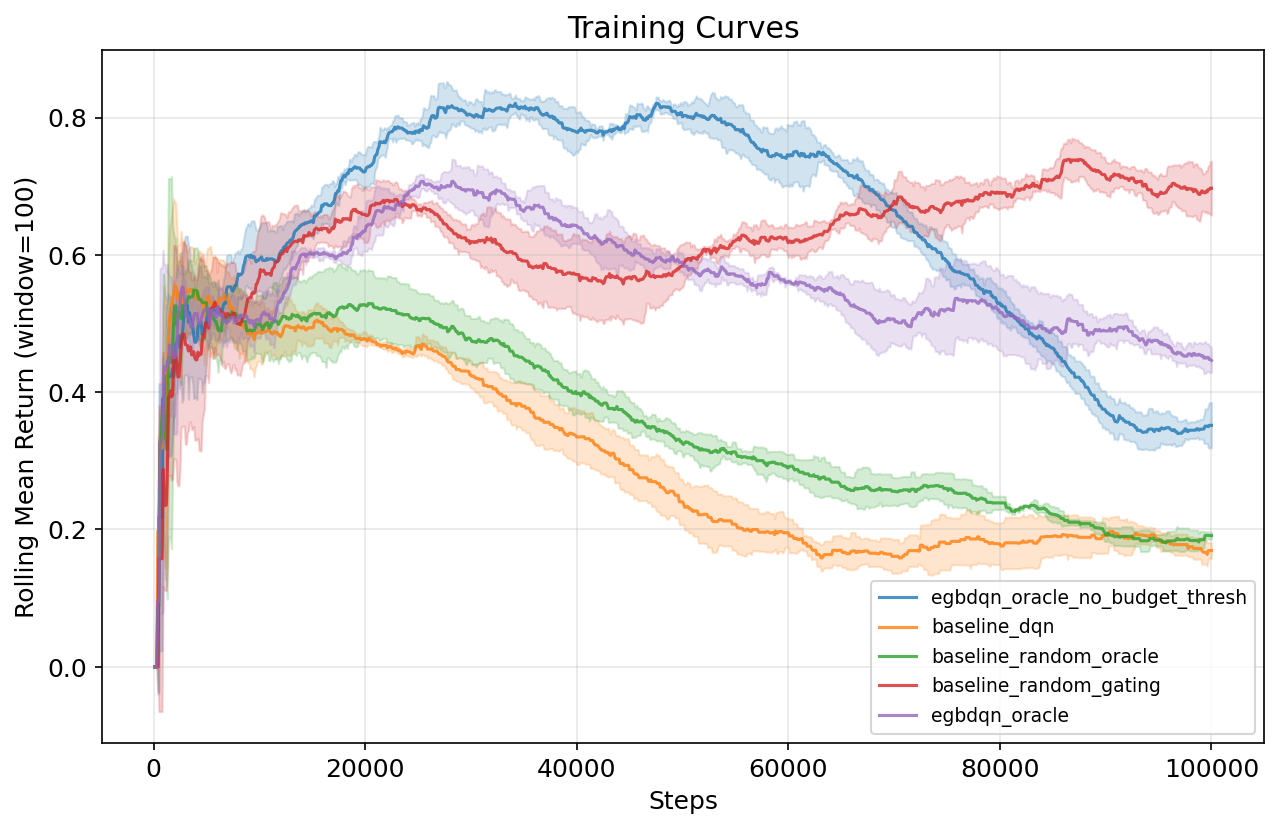
\includegraphics[width=\textwidth]{./images/training_curves.png}
        \caption{Rolling Mean Return}
        \label{fig:training_curves}
    \end{subfigure}
    \hfill
    \begin{subfigure}[b]{0.48\textwidth}
        \centering
        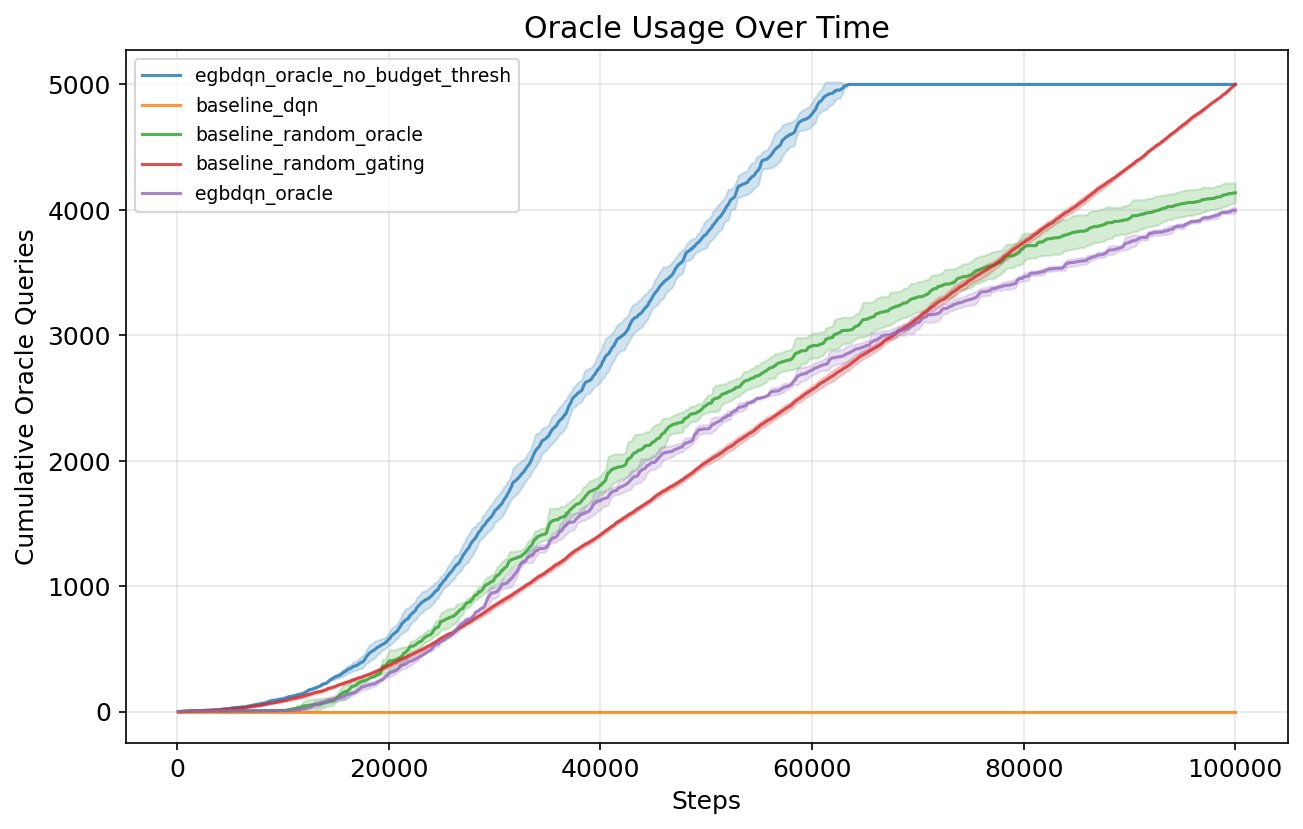
\includegraphics[width=\textwidth]{./images/oracle_usage.png}
        \caption{Cumulative Oracle Queries}
        \label{fig:oracle_usage}
    \end{subfigure}
    \caption{Round 1\&2 Training Dynamics. \textbf{(a)} EG-BDQN exhibits a gradual performance decay compared to the random gating baseline. \textbf{(b)} The epistemic gate prematurely shuts off, consuming queries early and then plateauing, while random gating provides a continuous minimum supervision floor.}
    \label{fig:round1_dynamics}
\end{figure}


\subsection{Round 2: Mixture Gating and the Budget Exhaustion Collapse}
\label{sec:round2}

To combat premature gate closure, we implemented two targeted fixes:
\begin{itemize}[leftmargin=*]
    \item \textbf{Minimum Query Floor.} A stochastic supervision floor ensures the oracle is queried with probability $p_{\mathrm{floor}} = 0.05 \cdot (B_{\mathrm{remaining}} / B)$ regardless of the uncertainty estimate, preventing full disconnection.
    \item \textbf{Mixture Gating.} The oracle is queried when \textit{either} the epistemic uncertainty exceeds the dynamic percentile threshold \textit{or} the random floor fires. This combines adaptive, uncertainty-targeted querying with a guaranteed trickle of supervision.
\end{itemize}

\paragraph{Result.} Mixture gating succeeded in keeping the epistemic gate open longer and distributing oracle queries more evenly across training. The agent achieved \textbf{higher peak sample efficiency} than any previous condition, reaching its maximum rolling mean return faster than both the original EG-BDQN and the random gating baseline.

However, a qualitatively different failure emerged: \textbf{the moment the oracle budget was fully exhausted, performance collapsed sharply}---more steeply than the gradual drift observed in Round~1. The agent transitioned abruptly from high-reward oracle-assisted behavior to poor autonomous performance, with the rolling mean return dropping precipitously. This is not a recurrence of the gate closure problem (the gate remained open throughout the budget); it is a fundamentally different failure mode.


\subsection{Theoretical Diagnosis: Oracle-Induced Covariate Shift}
\label{sec:dagger}

The steep post-budget collapse is a strong signal of a \textbf{transition-distribution failure} (covariate shift), not a simple exploration failure. We identify four interacting mechanisms:

\paragraph{(i) Oracle-Corrected State Distribution Shift.}
During oracle-assisted training, the state visitation distribution $d_{\mathrm{train}}(s)$ is shaped by the oracle's corrections: the agent is repeatedly redirected away from failure states and toward goal-relevant trajectories. Once the budget is exhausted, the policy must execute autonomously under a deployment distribution $d_{\mathrm{deploy}}(s)$ that includes precisely the failure-prone regions the oracle had been correcting. The Q-values in these unseen regions are poorly calibrated, leading to compounding errors.

\paragraph{(ii) Sparse Reward Credit Assignment.}
In the \texttt{GoToDoor} environment, rewards are sparse and delivered only upon task completion. Oracle-assisted successes provide reward signal, but the agent learns \textit{local policy fragments} around these assisted trajectories rather than the underlying long-horizon exploration structure needed for autonomous navigation. The credit assignment problem is masked during assisted training but surfaces immediately upon budget exhaustion.

\paragraph{(iii) Optimistic Q-Value Bootstrapping.}
Bellman updates during oracle-assisted episodes propagate value through $Q(s, a_{\mathrm{oracle}})$ rather than $Q(s, a_{\mathrm{agent}})$. Over time, the value landscape becomes \textit{optimistic for autonomous execution}: the agent's Q-function implicitly assumes that an oracle will intervene at critical decision points, inflating the expected return of states that are only reachable with expert assistance. When the oracle disappears, the agent follows these optimistic Q-values into states it cannot recover from.

\paragraph{(iv) Replay Dominance of Assisted Trajectories.}
The permanent oracle replay buffer, designed to preserve high-value demonstrations, inadvertently exacerbates the distribution mismatch. The network continues to train on oracle-assisted transitions long after the budget is exhausted, reinforcing the oracle-dependent value landscape rather than adapting to autonomous execution dynamics.

\paragraph{Synthesis.}
These four mechanisms converge to a single diagnosis: we are effectively training under \textbf{mixed expert-agent behavioral control} but evaluating under \textbf{pure agent control}. This is a classic instance of the covariate shift problem formalized in the DAgger framework \cite{ross2011reduction}---the training distribution does not match the deployment distribution, and the discrepancy grows with the horizon of the task. The mixture gating fix resolved the \textit{gating dynamics} problem but exposed the deeper \textit{distributional} problem that was always latent in the architecture.

\begin{table}[h]
    \centering
    \caption{Comparison of failure modes across experimental rounds.}
    \label{tab:failure_comparison}
    \begin{tabular}{@{} l l l @{}}
        \toprule
        & \textbf{Round 1 (Gate Closure)} & \textbf{Round 2 (Covariate Shift)} \\
        \midrule
        \textbf{Root cause} & Uncertainty miscalibration & Distribution mismatch \\
        \textbf{Failure trigger} & Gate closes prematurely & Budget exhausts \\
        \textbf{Decay profile} & Gradual drift & Sharp collapse \\
        \textbf{Oracle budget at failure} & Partially remaining & Fully consumed \\
        \textbf{Theoretical framing} & Ensemble calibration & DAgger covariate shift \\
        \bottomrule
    \end{tabular}
\end{table}


% ─────────────────────────────────────────────────────────────────────────────
\section{Current Limitations and Next Steps}
\label{sec:limitations}
% ─────────────────────────────────────────────────────────────────────────────

We emphasize that these are \textbf{preliminary results} from a proof-of-concept implementation. Two rounds of experiments have progressively clarified the core research problem. Round~1 identified premature gate closure as a gating dynamics issue; Round~2's mixture gating fix resolved this but revealed the deeper challenge of \textbf{oracle-induced covariate shift}. The central research question has accordingly shifted from ``how to keep the epistemic gate open'' to \textbf{``how to safely transition from oracle-assisted mixed control to pure autonomous execution.''}

\subsection{Immediate Research Priorities}

\begin{enumerate}[leftmargin=*, label=(\roman*)]
    \item \textbf{Conservative Q-Learning (CQL) regularization.} To counteract the optimistic Q-value bootstrapping identified in \Cref{sec:dagger}, we will investigate adding a CQL-style penalty that suppresses Q-values for out-of-distribution autonomous actions. This directly addresses the inflated value landscape by ensuring that states reachable only with oracle assistance are not assigned unrealistically high values under the autonomous policy.

    \item \textbf{DAgger-style rollout mixing.} Rather than a hard transition from mixed control to autonomous execution at budget exhaustion, we will explore a gradual handoff: as the budget depletes, the agent increasingly executes full autonomous rollouts while the oracle provides corrective labels on the agent's own state visitation distribution. This directly addresses the $d_{\mathrm{train}} \neq d_{\mathrm{deploy}}$ mismatch.

    \item \textbf{Autonomous validation phases.} We will introduce periodic oracle-free evaluation windows during training---before the budget is exhausted---to detect distributional fragility early. If autonomous performance degrades significantly relative to assisted performance, the system can reallocate remaining budget toward corrective demonstrations in the agent's own failure states rather than the oracle's preferred trajectories.

    \item \textbf{Architectural and calibration refinements.} The Round~1 findings remain relevant: shared-encoder head decoupling, MC-Dropout as an alternative uncertainty metric, and rigorous hyperparameter sweeps (rolling buffer size, percentile threshold, bootstrap mask probability) are needed to ensure the epistemic gate itself remains well-calibrated throughout training.
\end{enumerate}

\subsection{Roadmap: LLM Oracle Integration}

The current surrogate oracle (BabyAI heuristic bot) isolates the gating and transfer mechanisms from language-model-specific noise. Critically, solving the covariate shift problem in this controlled setting is the \textit{exact prerequisite} for safe LLM integration: an LLM oracle will introduce additional challenges (stochastic advice quality, latency, prompt sensitivity), but the distributional transfer problem is identical in structure. The roadmap proceeds as follows:

\begin{enumerate}[leftmargin=*, label=(\roman*)]
    \item \textbf{Stabilize autonomous transfer.} Validate CQL regularization and DAgger-style mixing on the heuristic oracle to achieve robust post-budget performance.
    \item \textbf{LLM-as-Oracle.} Replace the heuristic bot with a language model (e.g., GPT-4, Llama) that receives the mission string and a textual observation description. Characterize the interaction between LLM error rates and the covariate shift dynamics.
    \item \textbf{Scaling to harder environments.} Extend to multi-room BabyAI tasks (\texttt{KeyCorridor}, \texttt{PutNextLocal}) that require compositional reasoning and long-horizon planning, where the covariate shift is expected to be more severe and the value of principled transfer methods more pronounced.
\end{enumerate}


% ─────────────────────────────────────────────────────────────────────────────
\section{Conclusion}
% ─────────────────────────────────────────────────────────────────────────────

EG-BDQN proposes a principled framework for budget-constrained oracle supervision in reinforcement learning, leveraging ensemble disagreement to allocate expert queries to states of genuine epistemic ignorance. Two rounds of preliminary experiments have progressively sharpened our understanding of the architecture's core challenges.

Round~1 identified premature epistemic gate closure---a self-reinforcing failure cascade driven by shared-encoder Q-head convergence---and the contrast with random gating revealed that continuous supervision, even if budget-inefficient, provides critical stability. Round~2's mixture gating fix resolved the gating dynamics but exposed a deeper failure: oracle-induced covariate shift, wherein training under mixed expert-agent control produces a value function that is systematically miscalibrated for autonomous deployment. The sharp post-budget collapse is a classic DAgger-style distributional mismatch, not a simple exploration failure.

These findings reframe the core research problem from uncertainty calibration to \textit{safe policy transfer}. The identified failure modes are well-characterized, theoretically grounded, and suggest concrete mitigation strategies---Conservative Q-Learning, DAgger-style rollout mixing, and autonomous validation phases---that directly target the distributional gap. We believe this diagnostic trajectory, combined with the remediation roadmap, demonstrates that the EG-BDQN framework warrants further investigation as a scalable, budget-aware interface between RL agents and expensive external advisors, including LLMs.

\bibliographystyle{plainnat}
\bibliography{refs}

\end{document}
